\documentclass[a4paper,11pt]{scrartcl}
%\documentclass[a4paper,11pt]{exercice_sheet}
%\documentclass[a4paper,10pt]{article}
\usepackage[utf8x]{inputenc}
\usepackage[T1]{fontenc} % avec T1 comme option  d'encodage c'est ben mieux, surtout pour taper du français.
\usepackage{lmodern,textcomp} % fortement conseillé pour les pdf. On peut mettre autre chose : kpfonts, fourier,...
\usepackage[french]{babel} %Sans ça les guillemets, amarchpo
\usepackage{amsmath}
\usepackage{multicol}
\usepackage{amssymb}
\usepackage{tkz-tab}
\usepackage{exercice_sheet}

% Title Page
\title{Révisions BTS}
\subtitle{Corrigé des exercices}
\author{Patrick Augeau}

\begin{document}

\maketitle

%\begin{multicols}{2}

\section*{Calcul algébrique}

\exo{Développer et simplifier:}


$$A = (2x+3) (5x-2)$$
$$\Leftrightarrow A = 10x^2 - 4x + 15x - 6$$
$$\Leftrightarrow A = 10x^2 + 11x - 6$$

\trait

$$B = 2(x+5) 4(x+7)$$
$$\Leftrightarrow B = (2x + 10) + (4x + 28)$$
$$\Leftrightarrow B = 2x + 10 + 4x + 28$$
$$\Leftrightarrow B = 6x + 38$$

\trait

$$C = (3x+3)^2 - (4x+3)(4x-3)$$

On reconnaît ici:

\begin{itemize}
\item avant le signe $-$ l'identité remarquable $(a+b)^2 = a^2 + 2ab + b^2$
\item après le signe $-$ l'identité remarquable $(a+b)(a-b) = a^2 - b^2$
\end{itemize}


On obtient donc:

$$C = (3x)^2 + 2 \times 3x \times 3 + 3^2 - ((4x)^2 - 3^2)$$
$$C = 9x^2 + 18x + 9 - (16x^2 - 9)$$
$$C = 9x^2 + 18x + 9 - 16x^2 + 9$$
$$C = -7x^2 + 18x + 18$$



\exo{Factoriser}

$$A = (x+1)(3x+5) + (2x-7)(x+1)$$

On reconnaît ici que $(x+1)$ est facteur commun. On obtient donc
$$A = (x+1)(3x+5+2x-7)$$
$$A = (x+1)(5x-2)$$

\trait

$$B = 25x^2 - 49$$

On remarque qu'il s'agit d'une soustraction de deux carrés. Ceci correspond à l'identité remarquable $(a+b)(a-b) = a^2 - b^2$. $B$ se factorise donc de la façon suivante:

$$B = (5x+7)(5x-7)$$

\trait

$$C = 4x^2 - 4x + 1$$
$$C = (2x)^2 - 2 \cdot 2x \cdot 1 + 1^2$$

Il s'agit de l'identité remarquable $(a+b)^2 = a^2 + 2ab + b^2$. Il suffit donc de l'appliquer :
$$C = (2x-1)^2$$



\section*{Fractions}

\exo{Calculer}

$$A = \frac{1}{2} + \frac{1}{3}$$
$$A = \frac{3}{6} + \frac{2}{6}$$
$$A = \frac{3+2}{6} = \frac{5}{6}$$

\trait

$$B = \frac{2}{7} - \frac{5}{11}$$
$$B = \frac{22}{77} - \frac{35}{77}$$
$$B = \frac{-13}{77}$$

\trait

$$B = \frac{2}{7} \times \frac{3}{2}$$
$$B = \frac{2 \times 3}{7 \times 2}$$
$$B = \frac{6}{14}  = \frac{3}{7}$$


\trait

$$A = \frac{2}{x} - \frac{3}{x+1}$$
$$A = \frac{2(x+1)}{x(x+1)} - \frac{3x}{x(x+1)}$$
$$A = \frac{2(x+1) - 3x}{x(x+1)}$$
$$A = \frac{2x+2 - 3x}{x(x+1)} = \frac{-x+2}{x(x+1)}$$


\section*{Équations, inéquations, systèmes d'équations du 1\textsuperscript{er} degré}

\exo{Résoudre les équations suivantes:}


$$4x+5 = 7x+3$$
$$\Leftrightarrow 2 = 3x$$
$$\Leftrightarrow x = \frac{2}{3}$$
\trait
$$(5x-6)(5x+3) = 0$$

$$\Leftrightarrow 
\begin{cases}
5x-6 &= 0 \Leftrightarrow x = \frac{6}{5}\\ 
\mbox{ou}\\
5x+3 &= 0 \Leftrightarrow x = \frac{-3}{5}
\end{cases}$$
\trait
$$\frac{2x+5}{3} = \frac{x-1}{4}$$
$$\Leftrightarrow \frac{2}{3}x + \frac{5}{3} = \frac{x}{4} - \frac{1}{4}$$
$$\Leftrightarrow \frac{2x}{3} - \frac{x}{4} = - \frac{1}{4} - \frac{5}{3}$$
Mise au même dénominateur:
$$\Leftrightarrow \frac{8x - 3x}{12} = \frac{-3 - 20}{12}$$
$$\Leftrightarrow \frac{5x}{12} = \frac{-23}{12}$$
$$\Leftrightarrow 5x = -23 \Leftrightarrow x = \frac{-23}{5}$$
\trait
$$\frac{x}{3} + 7 = \frac{2x}{5} - \frac{3}{2}$$

Ici, on souhaite mettre 3 fractions au même dénominateur. Leurs dénominateurs respectifs sont 3, 5 et 2. Chaque fraction est alors multipliée par par ne dénominateur des deux autres. Par exemple $\frac{x}{3}$ est multipliée par 5 puis par 2, donc par 10. On obtient ainsi:
$$\frac{10x}{30} + \frac{210}{30} = \frac{12x}{30} - \frac{45}{30}$$
$$\Leftrightarrow 10x + 210 = 12x - 45$$
$$\Leftrightarrow 2x = 210+ 45$$

Soit: $x = \dfrac{255}{2}$




\exo{Résoudre les inéquations suivantes:}


$$x-14 > 7x+5$$
$$\Leftrightarrow x-7x > -5+14 \Leftrightarrow -6x > 9$$
C'est un nombre négatif ($-6$) qui a changé de côté, l'inégalité change donc de sens.
$$\Leftrightarrow x < -\frac{9}{6}$$
\trait
$$2x + 3 < 9x - 4 \Leftrightarrow 3+4 < 9x - 2x$$
$$\Leftrightarrow 7 < 7x \Leftrightarrow 1 < x$$


\section{Équations, inéquations du 2\textsuperscript{nd} degré}
\exo{$f(x) = 3x^2 + 5x - 2$}

\subquestion{Résoudre $f(x) = 0$}

$f(x) = 3x^2 + 5x - 2$. Il s'agit d'un polynôme du second degré. Résoudre $f(x) = 0$ revient donc à trouver les racines d'un polynôme du second degré.

On calcule dans un premier temps le $\Delta$ afin de connaître le nombre de racines.

$\Delta = 5^2 - 4 \times 3 \times (-2) = 25 + 24 = 49$


$\Delta > 0$, le polynôme a donc \textbf{2 racines}\footnote{on aurait pu écrire \og L'équation $f(x) = 0$ a 2 solutions. \fg{} Les 2 phrases sont parfaitement équivalentes.}.

$\sqrt{\Delta} = 7$

$x_1 = \frac{-5-7}{6} = -2$ et 
$x_2 = \frac{-5+7}{6} = \frac{1}{3}$

\subquestion{Factoriser $f(x)$}

Rappel : un polynôme de la forme $ax^2 + bx + c$ de racines $x_1$, $x_2$ se factorise sous la forme : $a(x-x_1)(x-x_2)$.

On a donc $f(x) = 3(x+2)\left(x-\dfrac{1}{3}\right)$.

\subquestion{Signe de $f(x)$ sur $\mathbb{R}$:}

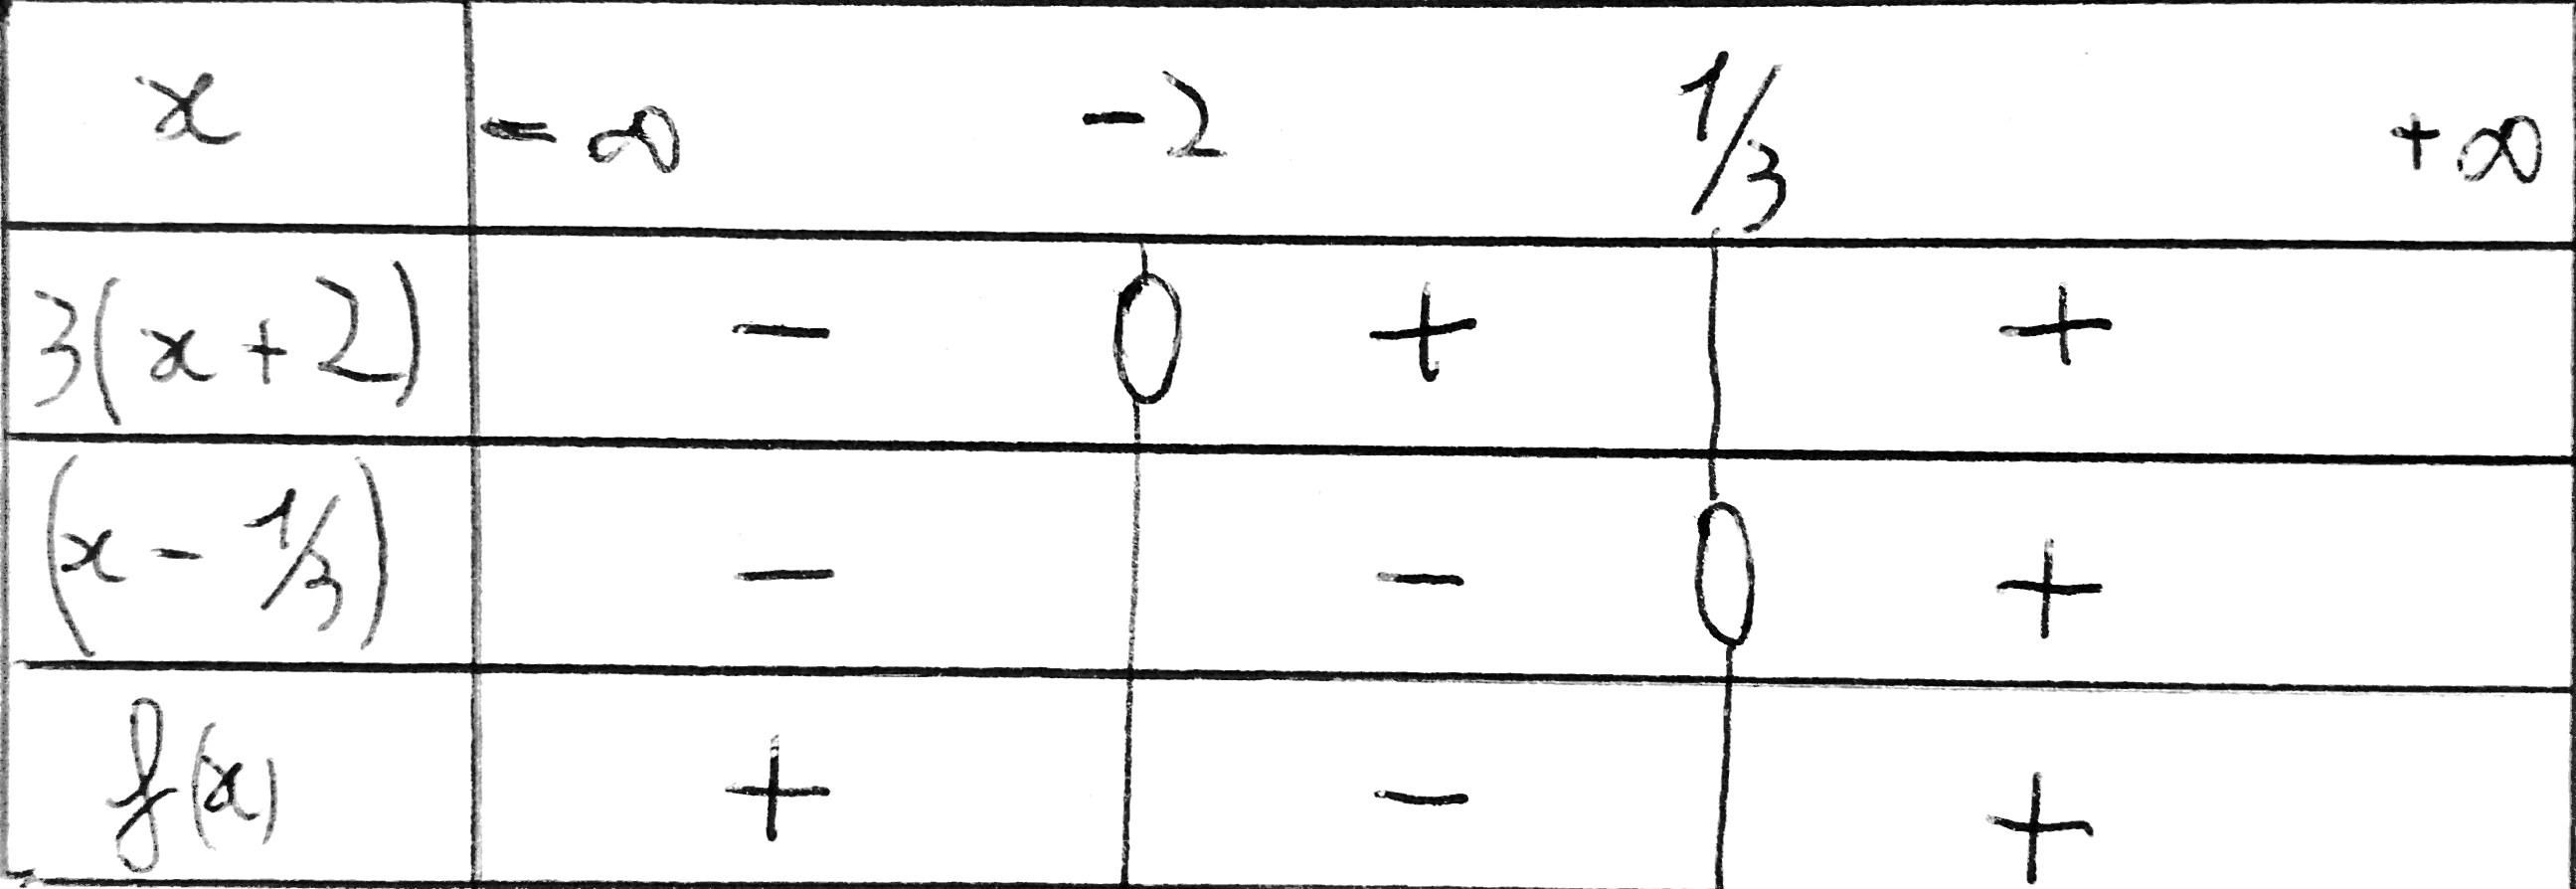
\includegraphics[width=0.5\textwidth]{pic/tab_sign_1.png}

\exo{$f(x) = x^2 - 2x + 3$}

Il s'agit d'un polynôme du second degré. On calcule donc $\Delta$: %Dans ce cas, $a = 1$ donc 

$\Delta = b^2 - 4ac$ donc ici : $\Delta = (-2)^2 - 4 \times 1 \times 3 = -8 < 0$

Le polynôme n'a pas de racine, il est donc du signe de $a$ sur $\mathbb{R}$.

Ici, $a = 1 > 0$ donc $f(x)$ est positive sur $\mathbb{R}$.

\section*{Fonction}

\question{}

$$f(1) = 2 \times 1^3 + 3 \times 1^2 - 12 \times 1 - 5 = -16$$ 
$$f(0) = 2 \times 0^3 + 3 \times 0^2 - 12 \times 0 - 5 = -5$$

\question{}
Voir graphe

\question{}
Voir graphe

\question{}
Voir graphe

\question{}

Voici le tableau de variation de la fonction $f$:

\begin{figure}
\begin{center}
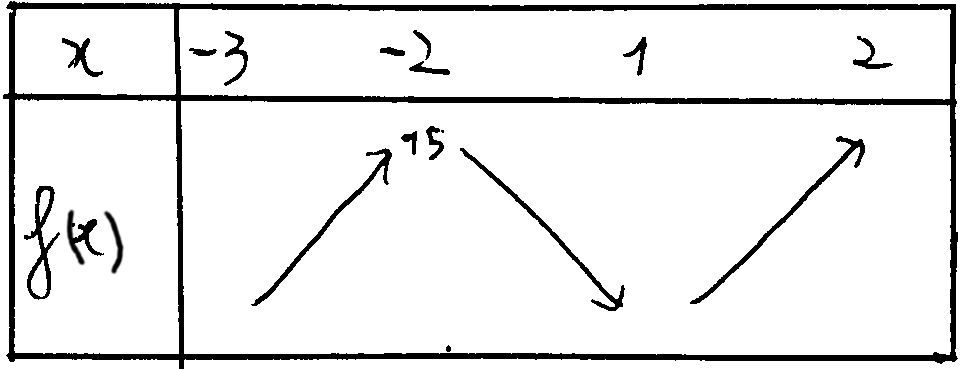
\includegraphics[width=0.5\textwidth]{pic/function_tab_var.png}
\end{center}
\caption{Tableau de variation de $f$}
\end{figure}


\begin{figure}
\includegraphics[width=1\textwidth]{pic/fonction.pdf}
\label{graphReponse}
\caption{Graphe}
\end{figure}

\section*{Fonction affine}

\exo{}

\question{}
Ici, attention à ne pas se laisser tromper par les échelles du graphe qui ne sont pas les mêmes en abscisse et en ordonnée. La lecture du coefficient directeur peut être faussée.

On peut lire sur le graphe que l'ordonnée à l'origine de la droite, $b$, est 4.

À ce stade, on sait que l'équation de la droite s'écrit $y = ax+4$. Il nous reste donc à trouver $a$.

On constate que la droite passe également par le point de coordonnées $(2;0)$.

En remplaçant $x$ et $y$, on obtient l'équation $0 = a \times 2 + 4 \Leftrightarrow a = -2$

L'équation de la droite est donc $y = -2x+4$

\question{}
Réponse sur le graphe.

\question{}
Réponse sur le graphe.

\begin{figure}
\begin{center}
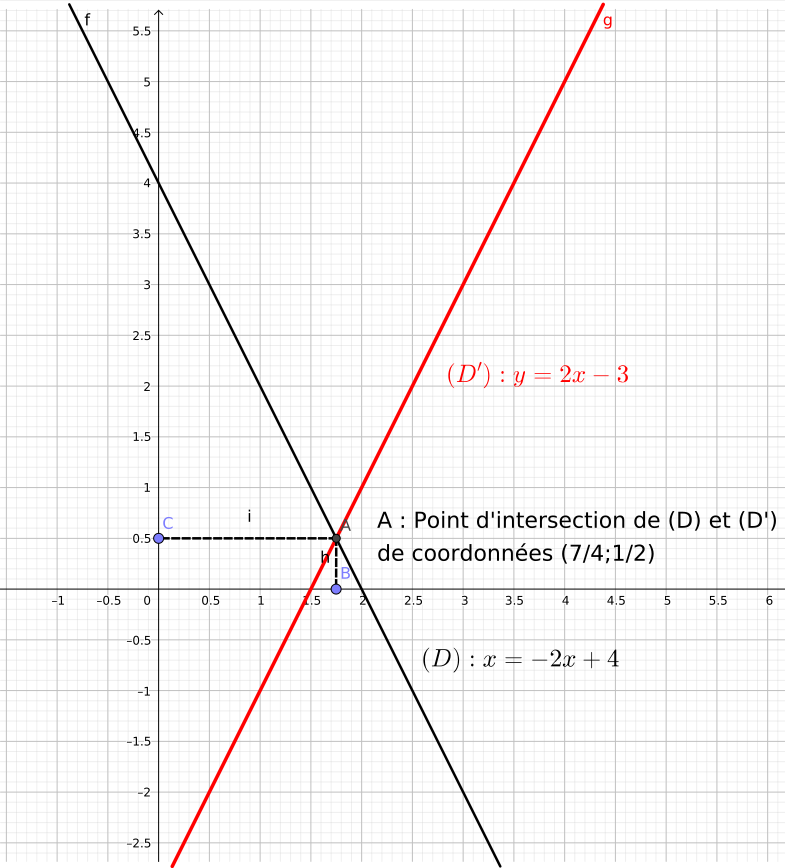
\includegraphics[width=0.8\textwidth]{pic/affine.pdf}
\end{center}
\caption{Fonctions affines}
\end{figure}

\question{Retrouver les résultats de la question précédente par le calcul:}

Les coordonnées du point d'intersection des 2 droites sont les solutions d'un système de 2 équations à 2 inconnues dont les équations sont les équations des droites. 

Ainsi, on doit résoudre le système 
$
\begin{cases}
y &= 2x-3\\ 
y &= -2x+4
\end{cases}
$
d'inconnues $x$ et $y$.

On constate qu'en additionnant les 2 équations, $x$ disparaît. On obtient donc: 

$2y = -3+4 \Leftrightarrow y = \dfrac{1}{2}$

En remplaçant $y$ par sa valeur dans une des équations du système de départ :

$\dfrac{1}{2} = 2x-3 \Leftrightarrow x = \dfrac{7}{4}$

Les coordonnées du point d'intersection sont donc $\left(\dfrac{7}{4};\dfrac{1}{2}\right)$

\question{Déterminer l'équation de la droite passant par 2 points de coordonnées M(1;8) et N(3;14)}

C'est une équation de droite que l'on cherche, donc elle est de la forme $y = ax+b$. On cherche à déterminer $a$ et $b$. Chacun des 2 points données dans l'énoncé va nous donner une équation. Cela va donc déboucher sur un système de 2 équations à 2 inconnues. 

\begin{itemize}
\item première équation: on remplace $x$ et $y$ par les coordonnées du point M : $8 = a+b$
\item deuxième équation: on remplace $x$ et $y$ par les coordonnées du point N : $14 = 3a+b$
\end{itemize}

On obtient donc le système: 
$
\begin{cases}
a+b &= 8\\ 
3a+b &= 14
\end{cases}
$.
En multipliant la ligne du haut par $-1$, on obtient: 
$
\begin{cases}
-a-b &= -8\\ 
3a+b &= 14
\end{cases}
$, et en additionnant les 2 lignes $b$ disparaît:

$2a = 6$ soit $a = 3$.

En injectant ce résultat dans la première équation, on obtient $3+b = 8$ soit $b = 5$.

L'équation de la droite (MN) est donc $y = 3a+5$.

\trait

%\end{multicols}
\end{document}
